% LATS 2027 submission draft. Every result is a \v... macro from generated/values.tex, written by
% analysis/run_all.py from the raw data in ../data. Do not type results by hand.
\documentclass[conference]{IEEEtran}
\usepackage{cite}
\usepackage{amsmath,amssymb}
\usepackage{graphicx}
\usepackage{booktabs}
\usepackage{xcolor}
\usepackage{tikz}
\usetikzlibrary{arrows.meta,positioning,calc}
\usepackage[hidelinks]{hyperref}
\usepackage{microtype}
\graphicspath{{figures/}}
\newcommand{\pending}[1]{\textcolor{red}{\textbf{[#1]}}}
\newcommand{\Vcc}{V_\mathrm{CCINT}}
\newcommand{\Dst}{\Delta^{*}_\mathrm{STA}}
% generated by analysis/run_all.py -- do not edit
\newcommand{\vAlphaVt}{0.64}
\newcommand{\vChainStages}{160}
\newcommand{\vColdHi}{315}
\newcommand{\vColdLo}{168}
\newcommand{\vColdMid}{264}
\newcommand{\vColdT}{46}
\newcommand{\vColdTHi}{46}
\newcommand{\vColdTLo}{46}
\newcommand{\vColdTMid}{46}
\newcommand{\vDVminAlphaHi}{12.9}
\newcommand{\vDVminAlphaLo}{12.5}
\newcommand{\vDVminAlphaMid}{12.9}
\newcommand{\vDVminErrHi}{2}
\newcommand{\vDVminErrLo}{1}
\newcommand{\vDVminErrMid}{2}
\newcommand{\vDVminHi}{10}
\newcommand{\vDVminLo}{15}
\newcommand{\vDVminMid}{13}
\newcommand{\vDVminRangeHi}{15}
\newcommand{\vDVminRangeLo}{10}
\newcommand{\vDpsHi}{$-$71}
\newcommand{\vDpsHiAbs}{71}
\newcommand{\vDpsLo}{$-$250}
\newcommand{\vDpsLoAbs}{250}
\newcommand{\vDpsMid}{$-$125}
\newcommand{\vDpsMidAbs}{125}
\newcommand{\vDslackErrHi}{0.9}
\newcommand{\vDslackErrLo}{1.1}
\newcommand{\vDslackErrMid}{1.0}
\newcommand{\vDslackHi}{$-$4}
\newcommand{\vDslackHiAbs}{4}
\newcommand{\vDslackLo}{$-$14}
\newcommand{\vDslackLoAbs}{14}
\newcommand{\vDslackMid}{$-$7}
\newcommand{\vDslackMidAbs}{7}
\newcommand{\vDstMinAbs}{213}
\newcommand{\vErrRateMin}{5\times10^{-9}}
\newcommand{\vFitBias}{+36}
\newcommand{\vFitHalfW}{69}
\newcommand{\vFitIcpt}{+29}
\newcommand{\vFitInside}{7}
\newcommand{\vFitInsideA}{6}
\newcommand{\vFitInsideB}{1}
\newcommand{\vFitMissMax}{71}
\newcommand{\vFitN}{11}
\newcommand{\vFitNullRms}{117}
\newcommand{\vFitP}{0.001}
\newcommand{\vFitR}{0.84}
\newcommand{\vFitRawBiasAbs}{261}
\newcommand{\vFitResVfR}{$-$0.26}
\newcommand{\vFitRho}{0.78}
\newcommand{\vFitRhoP}{0.004}
\newcommand{\vFitRms}{74}
\newcommand{\vFitRmsA}{83}
\newcommand{\vFitRmsB}{62}
\newcommand{\vFitSlope}{0.86}
\newcommand{\vGuardDVfmV}{0.2}
\newcommand{\vGuardDesignSt}{14.0}
\newcommand{\vGuardHDVfmV}{6.5}
\newcommand{\vGuardHDesignSt}{7.0}
\newcommand{\vGuardHPredEarly}{1}
\newcommand{\vGuardHPtN}{127}
\newcommand{\vGuardHPtPs}{144}
\newcommand{\vGuardHPtSd}{0.43}
\newcommand{\vGuardHPtSt}{8.06}
\newcommand{\vGuardPairs}{11}
\newcommand{\vGuardPtN}{246}
\newcommand{\vGuardPtPs}{254}
\newcommand{\vGuardPtSd}{0.18}
\newcommand{\vGuardPtSt}{14.24}
\newcommand{\vGuardSizedPs}{362}
\newcommand{\vGuardSizedSet}{3}
\newcommand{\vHotMinusColdHi}{$-$10}
\newcommand{\vHotMinusColdHiAbs}{10}
\newcommand{\vHotMinusColdLo}{+18}
\newcommand{\vHotMinusColdLoAbs}{18}
\newcommand{\vHotMinusColdMid}{$-$1}
\newcommand{\vHotMinusColdMidAbs}{1}
\newcommand{\vHotTHi}{105}
\newcommand{\vHotTLo}{104}
\newcommand{\vHotTMid}{104}
\newcommand{\vKtHi}{$-$0.17}
\newcommand{\vKtLo}{+0.31}
\newcommand{\vKtMid}{$-$0.02}
\newcommand{\vMaxSteps}{440}
\newcommand{\vOffsetResMax}{5.5}
\newcommand{\vOffsetResRms}{4.2}
\newcommand{\vPostHi}{305}
\newcommand{\vPostLo}{186}
\newcommand{\vPostMid}{264}
\newcommand{\vPostNsHi}{5.4}
\newcommand{\vPostNsLo}{3.3}
\newcommand{\vPostNsMid}{4.7}
\newcommand{\vPostSdHi}{0.6}
\newcommand{\vPostSdLo}{0.8}
\newcommand{\vPostSdMid}{0.7}
\newcommand{\vPreHi}{309}
\newcommand{\vPreLo}{200}
\newcommand{\vPreMid}{271}
\newcommand{\vPreT}{104}
\newcommand{\vPreTHi}{104.5}
\newcommand{\vPreTLo}{103.5}
\newcommand{\vPreTMid}{103.4}
\newcommand{\vRunDurH}{214.6}
\newcommand{\vRunN}{772\,479}
\newcommand{\vRunOven}{93.9}
\newcommand{\vRunPsu}{1.49}
\newcommand{\vRunSlack}{278.5}
\newcommand{\vRunSlackNs}{4.97}
\newcommand{\vRunSlackSd}{3.1}
\newcommand{\vRunT}{125.0}
\newcommand{\vRunTsd}{1.8}
\newcommand{\vRunV}{1.400}
\newcommand{\vRunVsdmV}{1}
\newcommand{\vShiftErrmV}{0.9}
\newcommand{\vShiftResMax}{0.7}
\newcommand{\vShiftResRms}{0.4}
\newcommand{\vShiftmV}{14.3}
\newcommand{\vSlopeHi}{383}
\newcommand{\vSlopeLo}{917}
\newcommand{\vSlopeMid}{560}
\newcommand{\vSlopePsHi}{6.8}
\newcommand{\vSlopePsLo}{16.4}
\newcommand{\vSlopePsMid}{10.0}
\newcommand{\vStaDCPR}{154}
\newcommand{\vStaDU}{120}
\newcommand{\vStaDeltaFastHi}{0.53}
\newcommand{\vStaDeltaFastLo}{0.11}
\newcommand{\vStaDeltaHi}{0.89}
\newcommand{\vStaDeltaLo}{0.06}
\newcommand{\vStaStageFastPs}{115}
\newcommand{\vStaStageSlowPs}{196}
\newcommand{\vSweepHi}{1.10}
\newcommand{\vSweepLo}{0.89}
\newcommand{\vTapAEarly}{1}
\newcommand{\vTapALateSure}{3}
\newcommand{\vTapAMaxPs}{+335}
\newcommand{\vTapAMaxPsAbs}{335}
\newcommand{\vTapAMaxSt}{+18.8}
\newcommand{\vTapAMaxmV}{+20}
\newcommand{\vTapAMinPs}{$-$85}
\newcommand{\vTapAMinPsAbs}{85}
\newcommand{\vTapAMinSt}{$-$4.8}
\newcommand{\vTapAMinmV}{$-$6}
\newcommand{\vTapAN}{6}
\newcommand{\vTapASdMax}{0.3}
\newcommand{\vTapASweeps}{6}
\newcommand{\vTapASweepsMax}{6}
\newcommand{\vTapASweepsMin}{6}
\newcommand{\vTapBEarly}{0}
\newcommand{\vTapBLateSure}{4}
\newcommand{\vTapBMaxPs}{+27}
\newcommand{\vTapBMaxPsAbs}{27}
\newcommand{\vTapBMaxSt}{+1.5}
\newcommand{\vTapBMaxmV}{+3}
\newcommand{\vTapBMinPs}{$-$108}
\newcommand{\vTapBMinPsAbs}{108}
\newcommand{\vTapBMinSt}{$-$6.1}
\newcommand{\vTapBMinmV}{$-$11}
\newcommand{\vTapBN}{5}
\newcommand{\vTapBSdMax}{0.2}
\newcommand{\vTapBSweeps}{4}
\newcommand{\vTapBSweepsMax}{4}
\newcommand{\vTapBSweepsMin}{4}
\newcommand{\vTapDie}{97}
\newcommand{\vTapGEarly}{9}
\newcommand{\vTapGLateSure}{0}
\newcommand{\vTapGMaxPs}{+565}
\newcommand{\vTapGMaxPsAbs}{565}
\newcommand{\vTapGMaxSt}{+31.6}
\newcommand{\vTapGMaxmV}{+35}
\newcommand{\vTapGMinPs}{+148}
\newcommand{\vTapGMinPsAbs}{148}
\newcommand{\vTapGMinSt}{+8.3}
\newcommand{\vTapGMinmV}{+9}
\newcommand{\vTapGN}{11}
\newcommand{\vTapGSdMax}{1.6}
\newcommand{\vTapGSweeps}{2}
\newcommand{\vTapGSweepsMax}{2}
\newcommand{\vTapGSweepsMin}{2}
\newcommand{\vTapGhEarly}{2}
\newcommand{\vTapGhLateSure}{0}
\newcommand{\vTapGhMaxPs}{+160}
\newcommand{\vTapGhMaxPsAbs}{160}
\newcommand{\vTapGhMaxSt}{+8.9}
\newcommand{\vTapGhMaxmV}{+18}
\newcommand{\vTapGhMinPs}{+46}
\newcommand{\vTapGhMinPsAbs}{46}
\newcommand{\vTapGhMinSt}{+2.6}
\newcommand{\vTapGhMinmV}{+3}
\newcommand{\vTapGhN}{5}
\newcommand{\vTapGhSdMax}{2.6}
\newcommand{\vTapGhSweeps}{2}
\newcommand{\vTapGhSweepsMax}{2}
\newcommand{\vTapGhSweepsMin}{2}
\newcommand{\vTapKhi}{1.01}
\newcommand{\vTapKhiPs}{18}
\newcommand{\vTapKlo}{0.52}
\newcommand{\vTapKloPs}{9}
\newcommand{\vTapN}{23}
\newcommand{\vTapNlong}{21}
\newcommand{\vTapNoGEarly}{1}
\newcommand{\vTapNoGLateSure}{7}
\newcommand{\vTapNoGMaxPs}{+335}
\newcommand{\vTapNoGMaxPsAbs}{335}
\newcommand{\vTapNoGMaxSt}{+18.8}
\newcommand{\vTapNoGMaxmV}{+20}
\newcommand{\vTapNoGMinPs}{$-$108}
\newcommand{\vTapNoGMinPsAbs}{108}
\newcommand{\vTapNoGMinSt}{$-$6.1}
\newcommand{\vTapNoGMinmV}{$-$11}
\newcommand{\vTapNoGN}{11}
\newcommand{\vTapNoGSdMax}{0.3}
\newcommand{\vTapNoGSweeps}{5}
\newcommand{\vTapNoGSweepsMax}{6}
\newcommand{\vTapNoGSweepsMin}{4}
\newcommand{\vTapShmoos}{8}
\newcommand{\vTapSweepsPerS}{5,677}
\newcommand{\vTapVfHi}{0.912}
\newcommand{\vTapVfLo}{0.725}
\newcommand{\vTapVhi}{0.949}
\newcommand{\vTapVlo}{0.725}
\newcommand{\vUsDAHi}{+0.00}
\newcommand{\vUsDALo}{$-$0.48}
\newcommand{\vUsDAMid}{$-$0.06}
\newcommand{\vUsDBHi}{+0.00}
\newcommand{\vUsDBLo}{+0.00}
\newcommand{\vUsDBMid}{+0.00}
\newcommand{\vUsDmax}{0.5}
\newcommand{\vUsDmaxPs}{9}
\newcommand{\vUsDurH}{37.4}
\newcommand{\vUsOven}{85}
\newcommand{\vUsPathNs}{1.9}
\newcommand{\vUsPostAHi}{417.00}
\newcommand{\vUsPostALo}{408.24}
\newcommand{\vUsPostAMid}{411.13}
\newcommand{\vUsPostBHi}{415.00}
\newcommand{\vUsPostBLo}{405.00}
\newcommand{\vUsPostBMid}{411.00}
\newcommand{\vUsPreAHi}{417.00}
\newcommand{\vUsPreALo}{408.72}
\newcommand{\vUsPreAMid}{411.19}
\newcommand{\vUsPreBHi}{415.00}
\newcommand{\vUsPreBLo}{405.00}
\newcommand{\vUsPreBMid}{411.00}
\newcommand{\vUsSensA}{8.3}
\newcommand{\vUsStepPs}{19.84}
\newcommand{\vUsTA}{113}
\newcommand{\vUsTAHi}{61}
\newcommand{\vUsTALo}{61}
\newcommand{\vUsTAMid}{61}
\newcommand{\vUsTB}{169}
\newcommand{\vUsTBHi}{105}
\newcommand{\vUsTBLo}{104}
\newcommand{\vUsTBMid}{104}
\newcommand{\vUsTsdA}{1.3}
\newcommand{\vUsVA}{0.847}
\newcommand{\vWorstLatePs}{108}
\newcommand{\vWorstLateSt}{6.1}
\newcommand{\vWorstLatemV}{11}
\newcommand{\vZeroPtsMax}{2}


% Double-blind switch: set \blindtrue if the LATS 2027 call requires anonymous submission.
\newif\ifblind \blindfalse

\begin{document}

\title{How Far from Failure Is a Zero Slack Reading?\\ Predicting and Guard-Banding the Offset of
an FPGA Aging Sensor}

\ifblind
\author{\IEEEauthorblockN{Anonymous authors}\IEEEauthorblockA{Affiliation withheld for review}}
\else
% Author order set by the group on 2026-11-21.
\author{\IEEEauthorblockN{Arthur Pamplona\IEEEauthorrefmark{1}, Danilo Alencar\IEEEauthorrefmark{1},
Alisson Barros\IEEEauthorrefmark{1}, Lucas Nogueira\IEEEauthorrefmark{1},
Jarbas Silveira\IEEEauthorrefmark{1}, and Fabian Vargas\IEEEauthorrefmark{2}}
\IEEEauthorblockA{\IEEEauthorrefmark{1}Universidade Federal do Cear\'a (UFC), Fortaleza, Brazil\\
\IEEEauthorrefmark{2}IHP -- Leibniz Institute for High Performance Microelectronics, Frankfurt (Oder), Germany}}
\fi

\maketitle

\begin{abstract}
Silicon lifecycle management (SLM) acts on phase-swept slack sensors, yet whether a zero reading
marks the functional failure of the monitored path is rarely measured. We drive a tapped delay chain
on a 16\,nm Artix UltraScale+ FPGA through failure by lowering the core voltage, each tap carrying
the sensor and a functional checker on one capture flip-flop. On \vAllN{} failing taps in four
placements, the zero reading and the first error were $-$\vAllMinPsAbs{} to $+$\vAllMaxPsAbs\,ps of
slack apart (negative: error first). This offset is the sensor's own sampling skew: without the
analysis-only margins of its cross-clock path, static timing predicts it to \vAllRms\,ps rms
(\vAllNullRms\,ps for a constant), and to \vCDRms\,ps on two placements predicted before
measurement. A static phase on the system clock turns it into a designed guard band without moving
the failure voltage; sized from static timing, it would cover every measured tap. On a 28\,nm
Artix-7, a burn-in's slack loss on an adder path at three core voltages amounts to one supply shift
of \vShiftmV\,mV. A zero reading is a failure warning only once its offset is known: static timing
predicts it, and one voltage sweep measures it.
\end{abstract}

\begin{IEEEkeywords}
Aging sensor, timing margin, FPGA, functional failure, guard band, burn-in, silicon lifecycle
management
\end{IEEEkeywords}

% =============================================================================================
\section{Introduction}

On-chip monitors are moving from characterization chips into products, where SLM software reads
them to set adaptive voltage scaling (AVS), raise margin alarms and estimate remaining
life~\cite{kashyap21,niemann20,vargas25,lanzieri24}. A timing-margin sensor serves those loops only
if its reading means what they assume: that a zero reading marks the operating point at which the
monitored path starts to fail. Processors face the same question with replica monitors, which must
be matched to the paths they stand for: the critical-path monitor of POWER6 tracks the real paths to
within three FO2 delays~\cite{drake07} and drives guard-band management in POWER7~\cite{lefurgy11},
tunable replica circuits are trimmed to fail before the critical paths~\cite{tschanz09}, and
silicon odometers separate the aging mechanisms~\cite{keane10}. In situ, failure prediction from a
guard band ahead of the capture edge~\cite{agarwal07}, error-prediction flip-flops whose guard band
adapts to aging~\cite{martins11}, and error detection at the capture flip-flop~\cite{razor04} are
established. On FPGAs, aging sensors based on phase-shifted sampling have been validated under
stress~\cite{valdes13,sensible17}; clock-sweep self-measurement of path delays goes back to Wong
\textit{et al.}~\cite{wong09} and was used to track degradation~\cite{stott10}, as were ring
oscillators~\cite{amouri14}; online
slack measurement with phase-shifted shadow registers has driven voltage and frequency
scaling~\cite{levine14}; voltage scaling has been made safe by calibrating the actual failing points
of each application on each device~\cite{ahmed16}; and online delay monitors now reach every timing
path, with an average error of 1.5\,\%~\cite{jiang22}. These works track degradation, match a
monitor to its paths at test time, or measure the failure point itself; to our knowledge, none
measures, path by path, how far the zero reading of an in-situ sensor lies from the first
functional error of the path it watches, or predicts that distance from static timing.

A dynamic phase shift added to the sensor of~\cite{vargas24} lets it measure the slack of a path
continuously, without recalibration~\cite{sbcci25}. The question SLM needs answered remains open:
\emph{how far from failure is a path whose reading is zero?} The obstacle is practical: a path with
enough slack to be safe at the nominal point does not fail within the voltage range of a board, and
one path gives one failure point.

This paper answers the question with measurements on two FPGA generations:
\begin{enumerate}
\item A multi-endpoint test structure (Section~\ref{sec:struct}): taps of graded length on one
ripple chain, each with the sensor and a functional checker on the same capture flip-flop, so one
core-voltage sweep moves the failure boundary across many paths under the same conditions.
\item The answer on 16\,nm (Sections~\ref{sec:res16}--\ref{sec:guard}): over \vAllN{} taps in four
placements, the zero reading and the first error differ by $-$\vAllMinPsAbs{} to
$+$\vAllMaxPsAbs\,ps of slack, an offset that belongs to the sensor's implementation, not to the
path. Static timing analysis (STA) predicts it to \vAllRms\,ps rms once its analysis-only margins
are removed, also out of sample (\vCDRms\,ps on two placements predicted before they were
measured); it follows the clock and setup-time steps between taps but overstates their routing
part. A static clock phase moves the offset by design without touching the failure voltage, so the
guard band an SLM loop must add can be sized at design time and checked with one shmoo.
\item The margin a burn-in consumes, read through the sensor on 28\,nm (Section~\ref{sec:res28}):
the steps lost grow from \vDslackHiAbs{} at 1.1\,V to \vDslackLoAbs{} at 0.9\,V, yet one supply
shift of \vShiftmV\,mV reproduces all three corners, as a uniform threshold-voltage increase would;
the temperature coefficient of the reading changes sign near 1.0\,V. A \vUsDurH\,h stress of two
16\,nm boards at nominal voltage, by contrast, moved their readings by less than one step.
\end{enumerate}

% =============================================================================================
\section{Sensor and Reading}\label{sec:sensor}

The sensor~\cite{sbcci25} samples the monitored path with two flip-flops (Fig.~\ref{fig:struct}a):
FF2 on the system clock and FF1 on a clock whose phase the clock manager (MMCM) shifts at run
time. FF3 latches their XOR on a catcher clock a fixed fraction of the period later. A controller
moves the FF1 clock earlier one fine step at a time, $\delta\phi = 1/(56 f_\mathrm{VCO})$~\cite{ug572}
(17.857\,ps at $f_\mathrm{VCO}=1$\,GHz), and the reading $r$ is the first step at which the sensor
alarms. The path toggles every cycle, so the alarm is deterministic up to jitter.

\textbf{What a reading means.} Let $s_1$ and $s_2$ be the setup slacks of the path at FF1 (at phase
step 0) and at FF2 (Fig.~\ref{fig:struct}b). FF1 sees the previous value, and the alarm fires, once
$r\,\delta\phi > s_1$, so $r=\lceil s_1/\delta\phi\rceil$; the functional capture fails when $s_2<0$.
The two slacks differ by an implementation offset $\Delta=s_2-s_1$: the skew between the two clock
trees at FF1 and FF2, the routing from the path to each flip-flop, and their setup times. If
$\Delta>0$ the reading reaches zero while FF2 still captures correctly, a warning margin of $\Delta$;
if $\Delta<0$ the sensor is late, and the path fails while it still reads $|\Delta|/\delta\phi$
steps. In voltage the margin is $\Delta/|\partial d/\partial\Vcc|$, with $d$ the path delay.

\textbf{After failure.} Once a path fails ($T<d<2T$), FF1 and FF2 capture the same stale value at
step 0, and the next alarm appears only near $r=(2T-d)/\delta\phi$: beyond the sweep (no alarm) or as
a large, aliased reading. The same blindness applies to one edge: when the slower transition fails
at both flip-flops, the reading reflects the other edge. A reading alone cannot tell a failing path
from a safe one; a functional checker can.

% =============================================================================================
\section{Multi-Endpoint Test Structure}\label{sec:struct}

\begin{figure}[t]
\centering
\resizebox{\columnwidth}{!}{% Fig. 1: (a) multi-endpoint test structure, (b) timing of one tap (TikZ, one column)
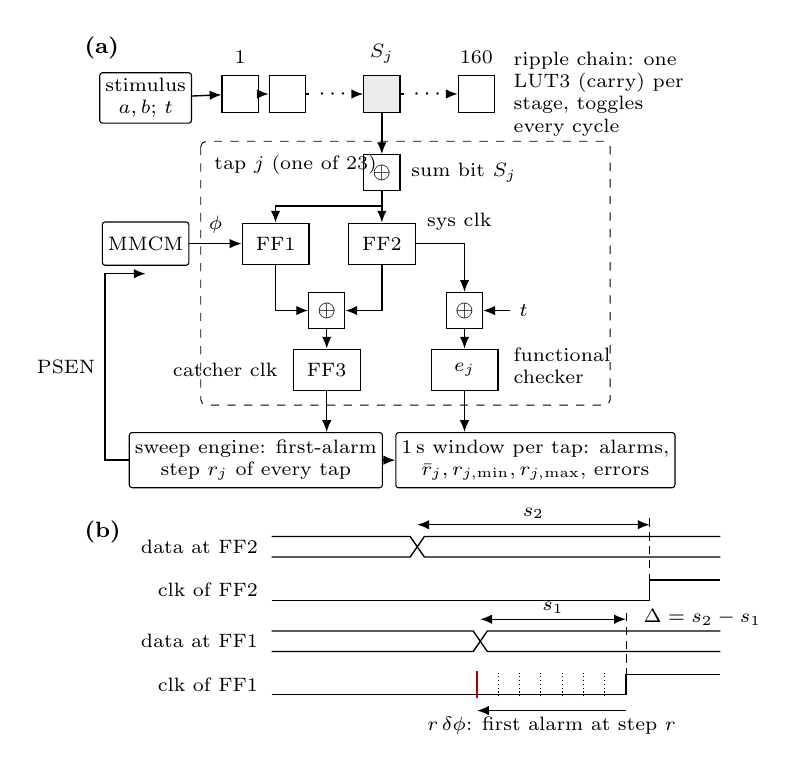
\begin{tikzpicture}[font=\footnotesize, >={Latex[length=1.5mm,width=1.2mm]}, x=1cm, y=1cm,
  lut/.style={draw, minimum width=4.6mm, minimum height=4.6mm, inner sep=0pt},
  ff/.style={draw, minimum width=8.5mm, minimum height=5.2mm, inner sep=0pt, font=\scriptsize},
  blk/.style={draw, rounded corners=1pt, inner sep=2pt, align=center, font=\scriptsize},
  lab/.style={font=\scriptsize},
  w/.style={->, line width=0.5pt}, l/.style={line width=0.5pt}]
% ================================================================ (a) structure
\node[font=\footnotesize\bfseries, anchor=south west] at (-0.75,0.32) {(a)};
\node[blk, minimum height=6mm] (stim) at (0.15,-0.05) {stimulus\\$a,b$; $t$};
\node[lut] (c1) at (1.35,0) {};
\node[lut] (c2) at (1.95,0) {};
\node (d1) at (2.55,0) {$\cdots$};
\node[lut, fill=black!8] (cj) at (3.15,0) {};
\node (d2) at (3.75,0) {$\cdots$};
\node[lut] (cn) at (4.35,0) {};
\draw[w] (stim) -- (c1); \draw[w] (c1) -- (c2); \draw[l] (c2) -- (d1); \draw[w] (d1) -- (cj);
\draw[l] (cj) -- (d2); \draw[w] (d2) -- (cn);
\node[lab, above=0.3mm of c1] {1};
\node[lab, above=0.3mm of cj] {$S_j$};
\node[lab, above=0.3mm of cn] {160};
\node[lab, anchor=west, align=left] at (4.7,0) {ripple chain: one\\LUT3 (carry) per\\stage, toggles\\every cycle};
% tap j
\draw[dashed, line width=0.35pt, rounded corners=2pt] (0.85,-0.6) rectangle (6.05,-3.95);
\node[lab, anchor=north west] at (0.9,-0.65) {tap $j$ (one of 23)};
\node[lut] (s) at (3.15,-1.0) {$\oplus$};
\draw[w] (cj) -- (s);
\node[lab, anchor=west] at (3.4,-1.0) {sum bit $S_j$};
\node[ff] (f1) at (1.8,-1.9) {FF1};
\node[ff] (f2) at (3.15,-1.9) {FF2};
\coordinate (sp) at (3.15,-1.42);
\draw[l] (s) -- (sp); \draw[w] (sp) -- (f2);
\draw[w] (sp) -| (f1);
\node[lut] (x) at (2.45,-2.75) {$\oplus$};
\draw[w] (f1) |- (x); \draw[w] (f2) |- (x);
\node[ff] (f3) at (2.45,-3.5) {FF3};
\draw[w] (x) -- (f3);
\node[lab, anchor=east] at (1.95,-3.5) {catcher clk};
\node[lut] (k) at (4.2,-2.75) {$\oplus$};
\draw[w] (f2.east) -| (k);
\node[lab] (t) at (4.95,-2.75) {$t$};
\draw[w] (t) -- (k);
\node[ff] (e) at (4.2,-3.5) {$e_j$};
\draw[w] (k) -- (e);
\node[lab, anchor=west, align=left] at (4.7,-3.45) {functional\\checker};
\node[lab, anchor=west] at (3.6,-1.62) {sys clk};
% clock manager and readout
\node[blk, minimum width=8mm, minimum height=5.5mm] (mm) at (0.15,-1.9) {MMCM};
\draw[w] (mm) -- (f1) node[midway, above, font=\scriptsize] {$\phi$};
\node[blk, minimum width=2.9cm, minimum height=7mm] (sw) at (1.55,-4.65) {sweep engine: first-alarm\\step $r_j$ of every tap};
\node[blk, minimum width=3.3cm, minimum height=7mm] (st) at (5.1,-4.65) {1\,s window per tap: alarms,\\$\bar r_j, r_{j,\min}, r_{j,\max}$, errors};
\draw[w] (f3) -- (f3 |- sw.north);
\draw[w] (e) -- (e |- st.north);
\draw[w] (sw) -- (st);
\draw[w] (sw.west) -- ++(-0.3,0) |- ([yshift=-1mm]mm.south) node[pos=0.25, left, font=\scriptsize] {PSEN};
% ================================================================ (b) timing of one tap
\begin{scope}[yshift=-5.75cm]
\node[font=\footnotesize\bfseries, anchor=north west] at (-0.75,0.45) {(b)};
% rows: data at FF2, clock of FF2, data at FF1, clock of FF1 (swept)
\def\xa{1.75} \def\xb{7.45}
\def\dtwo{3.6} \def\done{4.4} \def\etwo{6.55} \def\eone{6.25} \def\dphi{0.27}
% data waveforms (bus with a transition)
\foreach \y/\d/\nm in {0/\dtwo/{data at FF2}, -1.2/\done/{data at FF1}} {
  \draw[l] (\xa,\y+0.13) -- (\d-0.09,\y+0.13) -- (\d+0.09,\y-0.13) -- (\xb,\y-0.13);
  \draw[l] (\xa,\y-0.13) -- (\d-0.09,\y-0.13) -- (\d+0.09,\y+0.13) -- (\xb,\y+0.13);
  \node[lab, anchor=east] at (\xa-0.05,\y) {\nm};
}
% clock of FF2 (system clock) and of FF1 at phase step 0
\draw[l] (\xa,-0.68) -- (\etwo,-0.68) -- (\etwo,-0.42) -- (\xb,-0.42);
\node[lab, anchor=east] at (\xa-0.05,-0.55) {clk of FF2};
\draw[l] (\xa,-1.88) -- (\eone,-1.88) -- (\eone,-1.62) -- (\xb,-1.62);
\node[lab, anchor=east] at (\xa-0.05,-1.75) {clk of FF1};
% swept FF1 edges: one step earlier each; the first edge before the data transition alarms
\foreach \k in {1,...,6} { \draw[densely dotted, line width=0.4pt] (\eone-\k*\dphi,-1.9) -- (\eone-\k*\dphi,-1.6); }
\draw[line width=0.9pt, red!70!black] (\eone-7*\dphi,-1.92) -- (\eone-7*\dphi,-1.58);
\draw[->, line width=0.45pt] (\eone,-2.08) -- (\eone-7*\dphi,-2.08) node[midway, below=-0.4mm, font=\scriptsize] {$r\,\delta\phi$: first alarm at step $r$};
% slacks
\draw[<->, line width=0.45pt] (\dtwo,0.28) -- (\etwo,0.28) node[midway, above=-0.5mm, font=\scriptsize] {$s_2$};
\draw[densely dashed, line width=0.3pt] (\etwo,0.36) -- (\etwo,-0.42);
\draw[<->, line width=0.45pt] (\done,-0.92) -- (\eone,-0.92) node[midway, above=-0.5mm, font=\scriptsize] {$s_1$};
\draw[densely dashed, line width=0.3pt] (\eone,-0.84) -- (\eone,-1.62);
\node[lab, anchor=west] at (\eone+0.1,-0.9) {$\Delta=s_2-s_1$};
\end{scope}
\end{tikzpicture}
}
\caption{(a)~Test structure (16\,nm). A ripple chain whose carry toggles every cycle feeds 23 taps
($S_j=24$, 48, and 70 to 150 in steps of 4); each tap has the sensor of~\cite{sbcci25} and a checker
that compares the capture flip-flop FF2 with a replica $t$ of the stimulus. One phase sweep reads
every tap; the FPGA keeps 1\,s statistics per tap. (b)~Timing of one tap: FF1 and FF2 capture the
same transition with slacks $s_1$ and $s_2$, and each step moves the FF1 edge $\delta\phi$ earlier.
The reading reaches zero when $s_1$ does, the path fails when $s_2<0$: $\Delta$ is the margin left
at a zero reading.}
\label{fig:struct}
\end{figure}

The chain has \vChainStages{} stages, one LUT3 (carry majority) per stage. Operand $a$ alternates
between 0x55..55 and 0x55..56 and $b=$\,0xAA..AA, so every carry toggles each cycle and both edges
ripple through the whole chain.
Tap $j$ takes the sum bit of stage $S_j$ through its own LUT, so all taps load the chain alike. Two
control taps never fail; the other \vTapNlong{} are four stages apart. On this die, between
\vTapVhi{} and \vTapVlo\,V at the 10\,ns period, the failure boundary crosses \vTapAN, \vTapBN,
\vTapCN{} and \vTapDN{} of them in placements A to D (S\vTenStageLo{} to S\vTenStageHi); the longer ones already fail at
the top of the range, and a longer period brings them in (below). Each tap feeds a sensor and a
checker $e_j=\mathrm{FF2}_j\oplus t$, which is 0 in every
cycle while the tap meets timing; the checker is a short single-cycle path, so an error is the
monitored path's. A sweep engine moves the FF1 clock until every tap has alarmed or \vMaxSteps{}
steps (inside the catcher window) have passed, returns the phase to its origin and repeats, about
\vTapSweepsPerS{} times per second. For every 1\,s window and tap the FPGA keeps the number of sweeps
with an alarm, the mean, minimum and maximum reading, and the number of cycles with $e_j=1$; a
virtual I/O core clocked by the board oscillator exposes them to the JTAG.

\textbf{Implementation.} The design targets xcau15p-ffvb676-1-i (Vivado 2025.2). Chain, sensors and
checkers occupy one exclusive region; placements A to D put that region in four places of the die,
in different clock regions, which gives the same logic four different routings. Each tap path has a
reachable max-delay target (0.6\,ns + 0.15\,ns per stage) instead of the impossible 10\,ns
requirement. Two details matter for the sensor. First, Vivado models MMCM output phases as clock
latency, so by default it timed FF2$\rightarrow$FF3 against the \emph{next} catcher edge and padded
the route by 5\,ns to meet a spurious hold requirement, which would have shrunk the observation
window to about 3.8\,ns; a setup multicycle of 0 restores the same-edge capture (0.56\,ns of
routing). Second, the MMCM forbids a static phase on the output with fine phase shift, so the
sensor carries no designed guard band: $\Delta$ is whatever the implementation gives. STA reports
it per tap as the difference of the FF2 and FF1 setup slacks, \vStaDeltaLo{} to \vStaDeltaHi\,ns in
the slow corner, positive in \vStaDeltaPosN{} of the \vStaDeltaTaps{} taps of the four placements.

\textbf{Clock period.} Changing only the MMCM output dividers of a routed design runs it at 12 to
18\,ns with the same placement, routing and 1\,GHz VCO, so $\delta\phi$ is unchanged and the catcher
keeps its 1.75\,ns distance to FF2. The failure boundary then crosses longer taps inside the voltage
range, and STA of the variants gives the same offset per tap to within \vPeriodDstMaxPs\,ps.

% =============================================================================================
\section{Experimental Setup}\label{sec:setup}

\textbf{16\,nm.} The structure runs on an RV02A board (Artix UltraScale+ xcau15p, nominal
$\Vcc=0.85$\,V; board~2 of Section~\ref{sec:res16bound}) whose core rail comes from a TPS65400
regulator that an STM32 sets in 10\,mV steps; $\Vcc$ and the die temperature are read from the
SYSMON through the JTAG. Each shmoo steps $\Vcc$ from \vTapVhi{} down to \vTapVlo\,V and back (two
windows to settle, then 6 to 8 windows of $10^{8}$ cycles, 1\,s at 10\,ns, i.e.\ up to
$8\times10^{8}$ checked cycles per point; \vShmooMinLo{} to \vShmooMinHi\,min per shmoo), always
above the 0.72\,V operating point of the low-voltage grade of the family~\cite{ds931} and below its
1.0\,V absolute maximum. Two sessions \vSessGapDays{} days apart took \vShmoosFirst{} shmoos (A and B
at 10\,ns, and the guards of Section~\ref{sec:guard}) and \vShmoosSecond{} (A and B at 12 to 18\,ns,
C and D at 10, 14 and 18\,ns, and A again). The board sat at room temperature; its
SYSMON read about \vTapDie\,\textdegree C, a known offset of this board's sensor that we report but
do not use. The margins below are differences of readings in phase steps and do not depend on the
SYSMON voltage calibration, which enters only the voltages we quote.

\textbf{28\,nm.} A Nexys~4~DDR board (Artix-7 xc7a100t, nominal 1.0\,V) runs the same sensor, with
the same 17.857\,ps step, on the most significant sum bit of a 16-bit ripple-carry adder whose
inputs toggle every cycle. An IT6502D supply feeds the core rail and is trimmed every second against
the XADC reading of $\Vcc$; the board sits in an oven under PID control~\cite{sbcci26}. The burn-in
(Run~1) lasted \vRunDurH\,h at $\Vcc=\vRunV$\,V ($\pm$\vRunVsdmV\,mV) and a die temperature of
$\vRunT\pm\vRunTsd$\,\textdegree C (oven air \vRunOven\,\textdegree C), with the sensor read every
second (\vRunN{} samples) and never recalibrated; it read $\vRunSlack\pm\vRunSlackSd$ steps
(\vRunSlackNs\,ns of slack). At about \vPreT\,\textdegree C, corners at 1.10, 1.00 and 0.90\,V were
taken before the burn-in (single readings) and right after it, in a logged run that also stepped
$\Vcc$ from \vSweepHi{} to \vSweepLo\,V; cold corners at \vColdT\,\textdegree C followed. The burn-in
is a deliberate overstress (1.4\,V exceeds the absolute-maximum core voltage of the
Artix-7~\cite{ds181}), so the rates reported here do not transfer to product
burn-in~\cite{jesd22a108}.

% =============================================================================================
\section{Results}

\subsection{\texorpdfstring{16\,nm}{16 nm}: Zero Reading Versus First Error}\label{sec:res16}

\begin{figure}[t]
\centering
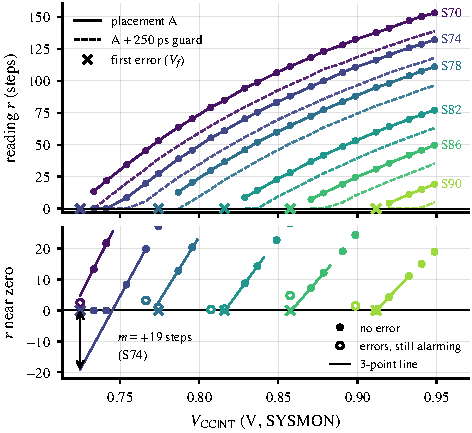
\includegraphics[width=\columnwidth]{fig_tap_shmoo}
\caption{16\,nm, one downward sweep of placement A at 10\,ns. Top: reading of the taps whose failure boundary
falls inside the sweep (solid) and of the same routed design with the 250\,ps guard of
Section~\ref{sec:guard} (dashed); a point is drawn while the tap's checker saw no error;
$\times$:~first failing voltage $V_f$. Bottom: close-up near zero. The line through the three
lowest error-free readings, extrapolated to the failure threshold, gives the margin $m$ (arrow:
S\vLooStage, which read zero at \vZeroPtsMax{} points before its first error); open circles: failing points at
which every sweep still alarmed.}
\label{fig:shmoo}
\end{figure}

Fig.~\ref{fig:shmoo} shows one downward voltage sweep. Near its failure boundary each tap's reading
falls almost linearly with $\Vcc$, at \vTapKlo{} to \vTapKhi{} steps per mV
(\vTapKloPs--\vTapKhiPs\,ps of slack per mV), and within one 10\,mV step the checker goes from no
error in up to $8\times10^{8}$ cycles to errors. Taps shorter than the boundary never erred, nor
did the control taps at any voltage. Longer taps erred in every cycle up to a delay of two periods,
beyond which the period-two stimulus makes a capture two cycles late look correct (the longest taps
at the lowest voltages); all showed either no alarm or the aliased reading of
Section~\ref{sec:sensor}. Error rates of exactly 0.5 between the two regimes show the two edges
failing at different voltages, and there the reading need not vanish: in every sweep,
\vHalfStages{} of placement \vHalfImpl{} still read \vHalfRLo{} to \vHalfRHi{} steps while one edge
failed in every cycle in which it occurred, the blindness to one edge of Section~\ref{sec:sensor}
(open circles in Fig.~\ref{fig:shmoo}).

For each failing tap and voltage sweep we fit a straight line to the three error-free, positive
readings closest to the boundary, extrapolate it to the failure threshold and call $m$ the negated
result, in ps: $m>0$ means the reading had reached zero before the first error. The threshold lies
between the first failing voltage $V_f$ and the last passing one; the bounds of $m$ that these two
voltages give are the error bars of Fig.~\ref{fig:offset} and the intervals of Table~\ref{tab:taps}.
As the best estimate we take $V_f$ when its error rate is below 0.5, since then only the jitter tail
of one edge fails there, and the middle of the interval otherwise. Fitting two or four points
instead of three changes $m$ by at most \vExtrapSensPs\,ps (\vExtrapSensGPs\,ps with the guard of
Section~\ref{sec:guard}, where the line runs beyond the data for up to \vTapGZeroPtsMax{} voltage
points). Over the \vAllSweepsMin{} to \vAllSweepsMax{} voltage sweeps of each tap (down and up,
repeated shmoos), $m$ varied by at most \vAllSdMax{} steps (standard deviation), or \vAllSdSplitMax{}
in \vAllVfSplit{} of the \vAllCases{} tap--period cases, whose sweeps first failed one 10\,mV step
apart.

Each tap enters the statistics once per placement, at the shortest period at which it fails inside
the range. Over these \vAllN{} independent taps, $m$ ranged from \vAllMinPs{} to \vAllMaxPs\,ps. No
tap read zero at more than \vAllZeroPtsMax{} voltage points before failing, and \vAllLateSure{} of
the \vAllN{} failed while still reading positive even at the favorable end of their interval, the
latest one (S\vAllMinStage{} of placement \vAllMinImpl{} at \vAllMinT\,ns) \vAllMinSt{} steps above
zero at the best estimate. The zero reading is thus a close but not a conservative predictor: as
built, the sensor can be late by up to \vAllMinPsAbs\,ps, or \vAllMinmV\,mV of core voltage.
Repeated \vSessGapDays{} days later with the same bitstream, the \vRepN{} taps of A moved their
margins by \vRepDLo{} to \vRepDHi\,ps (mean \vRepDMean\,ps) and kept their failure voltages to
within \vRepDVfmV\,mV.

\subsection{What Sets the Offset}\label{sec:offset}

\begin{figure}[t]
\centering
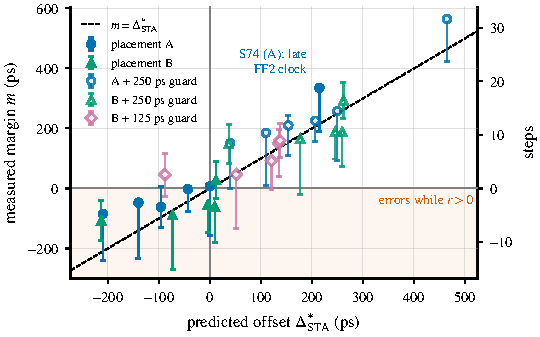
\includegraphics[width=\columnwidth]{fig_tap_offset}
\caption{Measured margin $m$ at failure versus the offset $\Dst$ predicted by STA without the
uncertainty and pessimism terms (slow corner), for the \vAllN{} independent taps of placements A to
D (taps per placement in parentheses). Filled: 10\,ns; hollow: the same routed designs at 12 to
18\,ns. Error bars span the 10\,mV interval in which errors start. Below zero the path fails while
the sensor still reads positive.}
\label{fig:offset}
\end{figure}

\begin{table}[t]
\centering
\caption{Per-tap results of the first session (16\,nm, 10\,ns): first failing voltage $V_f$ (V,
SYSMON), measured margin $m$ with its interval (super- and subscript) and predicted offset $\Dst$
(ps); $m'$, $m''$: margin of the same routed design with the 250 and the 125\,ps guard. $m>0$: the
reading reached zero before the first error. Means over \vTapASweeps{} (A), \vTapBSweeps{} (B) and
\vTapGSweeps{} (guards) voltage sweeps.}
\label{tab:taps}
\footnotesize
\setlength{\tabcolsep}{2.2pt}
% generated by analysis/tap_values.py -- do not edit
\begin{tabular}{@{}r@{\hspace{4pt}}ccc@{\hspace{5pt}}c@{\hspace{7pt}}ccc@{\hspace{5pt}}cc@{}}
\toprule
 & \multicolumn{4}{c}{placement A} & \multicolumn{5}{c}{placement B} \\
\cmidrule(lr){2-5}\cmidrule(lr){6-10}
$S$ & $V_f$ & $m$ & $\Dst$ & $m'$ & $V_f$ & $m$ & $\Dst$ & $m''$ & $m'$ \\
\midrule
70 & 0.725 & $-$85$^{\text{+0}}_{\text{$-$156}}$ & $-$210 & +151 & -- & -- & -- & -- & -- \\
74 & 0.725 & +335$^{\text{+0}}_{\text{$-$144}}$ & +215 & +565 & 0.754 & $-$89$^{\text{+0}}_{\text{$-$183}}$ & $-$73 & +46 & +165 \\
78 & 0.774 & $-$48$^{\text{+0}}_{\text{$-$185}}$ & $-$140 & +185 & 0.787 & $-$61$^{\text{+0}}_{\text{$-$120}}$ & +10 & +150 & +188 \\
82 & 0.816 & +7$^{\text{+0}}_{\text{$-$164}}$ & 0 & +257 & 0.829 & $-$56$^{\text{+0}}_{\text{$-$91}}$ & $-$4 & +92 & +190 \\
86 & 0.857 & $-$61$^{\text{+68}}_{\text{$-$68}}$ & $-$96 & +210 & 0.857 & $-$108$^{\text{+67}}_{\text{$-$67}}$ & $-$213 & +46 & +148 \\
90 & 0.912 & $-$3$^{\text{+0}}_{\text{$-$75}}$ & $-$43 & +226 & 0.899 & +27$^{\text{+61}}_{\text{$-$61}}$ & +12 & +160 & +293 \\
\bottomrule
\end{tabular}

\end{table}

The tap-to-tap spread follows the implementation. STA charges the FF1 path, which crosses from the
system clock into the phase-swept clock, \vAllDU\,ps more clock uncertainty and \vAllDCPRLo{} to
\vAllDCPRHi\,ps less clock-pessimism removal than the same-clock FF2 path; both are worst-case
analysis margins, not delays of a typical die. Removing both from the slack difference gives $\Dst$,
computed for each placement and period from its own routed design with no fitted parameter. This
correction was settled on the first session, where the \vSessN{} taps of A and B at 10\,ns followed it with
\vSessRms\,ps rms against \vSessNullRms\,ps for the best constant offset (Table~\ref{tab:sta}). Over
the \vAllN{} independent taps of both sessions (Fig.~\ref{fig:offset}), $\Dst$ predicts $m$ with
\vAllRms\,ps rms residual, against \vAllNullRms\,ps for the best constant ($r=\vAllR$, Spearman
$\rho=\vAllRho$, fitted slope \vAllSlope), or \vAllAltLongRms\,ps with each tap taken at its longest
period instead. The raw STA slack difference correlates as well ($r=\vAllRawR$) but would have
overstated the margins by \vAllRawBiasAbs\,ps on average, predicting a safe sensor where
\vAllLateBest{} taps were late; STA sets that shift without any measurement.

\begin{table}[t]
\centering
\caption{STA prediction of the margin, per set of independent taps: correlation $r$ and
least-squares slope of $m$ on $\Dst$, rms of $m-\Dst$ (no fitted parameter) and of $m$ about its
mean (the best constant). $^\dagger$\,$\Dst$ committed before the measurement.}
\label{tab:sta}
\footnotesize
\setlength{\tabcolsep}{3.5pt}
% generated by analysis/tap_values.py -- do not edit
\begin{tabular}{@{}lccccc@{}}
\toprule
Taps & $n$ & $r$ & slope & \multicolumn{2}{c}{rms (ps)} \\
\cmidrule(l){5-6}
 & & & & $m-\Dst$ & $m-\bar{m}$ \\
\midrule
Session 1: A, B at 10\,ns & 11 & 0.84 & 0.86 & 74 & 117 \\
Session 2: A, B at 12--18\,ns & 30 & 0.97 & 0.65 & 86 & 148 \\
Session 2: C, D$^\dagger$ & 40 & 0.94 & 0.95 & 70 & 199 \\
All & 81 & 0.93 & 0.81 & 77 & 175 \\
\midrule
Placement A & 21 & 0.95 & 0.62 & 97 & 148 \\
Placement B & 20 & 0.93 & 0.62 & 66 & 93 \\
Placement C & 20 & 0.91 & 0.77 & 69 & 135 \\
Placement D & 20 & 0.95 & 0.97 & 71 & 205 \\
\bottomrule
\end{tabular}

\end{table}

The second session tested the model out of sample. Its \vNewN{} new taps, the long taps of A and B
at 12 to 18\,ns and two new placements, C and D, whose $\Dst$ was committed to the project
repository before they were measured, follow $\Dst$ with \vNewRms\,ps rms against \vNewNullRms\,ps
for a constant (C and D alone: \vCDRms{} against \vCDNullRms\,ps), and in every placement STA beats
a constant offset (Table~\ref{tab:sta}). On the first session the correlation rested largely on one
tap: the FF2 of S\vLooStage{} in \vLooImpl{} receives the system clock \vClkOutPs\,ps later than the
other FF2s of S\vTapAStageLo--S\vTapAStageHi, and without it $r$ fell to \vLooR. Such clock steps turned out to be common, and STA
follows them: with the new taps, leaving out any one tap keeps $r$ between \vAllLooRLo{} and
\vAllLooRHi.

$\Dst$ has three parts, which the \vAllN{} taps separate: the arrival of the two capture clocks
(\vDecClkLo{} to \vDecClkHi\,ps, in steps that follow where FF1 and FF2 sit on their clock trees), the routing
from the tap to each flip-flop (\vDecRouteLo{} to \vDecRouteHi\,ps), and a \vDecSuPs\,ps smaller
setup time that STA assigns to FF2 at some slice locations (\vDecSuN{} taps of \vDecSuPl). The
silicon shows that last term: with it these taps miss $\Dst$ by \vDecSuRes\,ps on average, without
it by \vDecSuNoRes\,ps. A least-squares fit of $m$ to the three parts weights them \vDecCoClk,
\vDecCoSu{} and \vDecCoRoute{} (95\,\% bootstrap intervals \vDecCoClkLo--\vDecCoClkHi,
\vDecCoSuLo--\vDecCoSuHi{} and \vDecCoRouteLo--\vDecCoRouteHi; \vDecRms\,ps rms): the silicon
shows most of the clock and setup parts STA computes, but only about half of its routing
difference. The slope of $m$ on $\Dst$ within a placement, \vPlSlopeLo{} to \vPlSlopeHi,
depends on how much of its spread is routing.

STA gives the same $\Dst$ at every period, but the margin moves with the failure voltage. The
residual has no additive trend with it (correlation \vAllResVfR{} over \vAllVfLo--\vAllVfHi\,V),
yet the \vPairN{} pairs of measurements of one tap at two periods failed \vPairDVmV\,mV apart on
average and differed by \vPairDmPs\,ps in margin, and where the offset is large
($|\Dst|\ge100$\,ps) $|m|$ was larger at the lower voltage in \vPairBigGrow{} of \vPairBigN{} pairs:
the offset is a difference of delays and tends to grow with them toward low voltage, which a
single-corner STA cannot follow. $\Dst$ falls inside the measured interval for \vAllInside{} of the
\vAllN{} taps and misses the others by at most \vAllMissMax\,ps; the 10\,mV voltage grid alone
leaves an interval of $\pm$\vAllHalfW\,ps on average. STA thus gives the offset to about \vAllRms\,ps
before anything is measured, including its clock and setup steps; a tighter bound needs a
measurement.

\subsection{A Designed Guard Band}\label{sec:guard}

The MMCM accepts a static phase on the outputs without fine phase shift, in settings of one eighth
of the VCO period (125\,ps here). Delaying the system clock (launch registers, FF2 and checkers) by
9\textdegree{} (250\,ps) makes FF1 sample that much earlier at step 0 without touching the monitored
path. In the first session we applied it to the routed designs of A and B, changing nothing but two
MMCM attributes (A$'$, B$'$; the catcher keeps its distance to FF2). Two results were not given in
advance. At the \vGuardPtN{} tap--voltage points measured with and without it, the reading dropped
by \vGuardPtSt$\pm$\vGuardPtSd{} steps (\vGuardPtPs\,ps; designed \vGuardDesignSt), the same on every
tap to within the reading noise; and every tap first failed at the same 10\,mV step as before, so
the guard shifts the reading without loading the path. That all \vGuardPairs{} failing taps then
read zero before their first error, by \vTapGMinSt{} to \vTapGMaxSt{} steps (\vTapGMinPs{} to
\vTapGMaxPs\,ps) at the best estimate and \vTapGEarly{} of them even at the unfavorable end of their
interval, follows from \vGuardPtPs\,ps exceeding their latest offset of \vWorstLatePs\,ps. A single
setting (4.5\textdegree, B$''$) lowered the readings of B by \vGuardHPtSt$\pm$\vGuardHPtSd{} steps
(\vGuardHPtPs\,ps) instead of \vGuardHDesignSt, equally on every tap, and the second setting added
\vGuardStepTwoPs\,ps: the realized steps differ from the nominal 125\,ps, as a static phase offset
between MMCM outputs, which the data sheet bounds~\cite{ds931}, allows. With B$''$, all \vTapGhN{}
failing taps of B also read zero first, by \vTapGhMinPs{} to \vTapGhMaxPs\,ps (Table~\ref{tab:taps}).
The guard is thus a design parameter whose realized value must be measured once, as the reading
change of any tap with and without it.

A fixed guard does not carry over to other placements and periods, though. Shifted by the
\vGuardPtPs\,ps measured above, \vGuardFixLate{} of the \vAllCases{} tap--period cases would
still fail before reading zero, in placements \vGuardFixLatePl, whose offsets reach
\vAllMinPs\,ps. Sized per placement from STA alone, to cover the most negative $\Dst$ of its routed
design plus twice the rms error of the first session, the guard is \vGuardPlLo{} to
\vGuardPlHi\,ps (\vGuardPlSetLo{} to \vGuardPlSetHi{} settings), and shifted by it every one of the
\vAllCases{} cases would read zero at least \vGuardPlMinPs\,ps before its first error.

\subsection{\texorpdfstring{28\,nm}{28 nm}: The Margin a Burn-In Consumes}\label{sec:res28}

\begin{figure}[t]
\centering
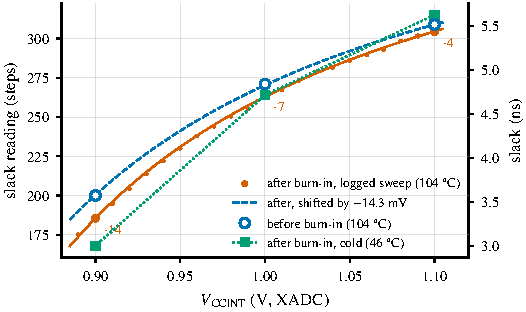
\includegraphics[width=\columnwidth]{fig_run1_corners}
\caption{28\,nm, 16-bit adder path. Slack reading versus core voltage after the \vRunDurH\,h burn-in
(logged sweep, marker area $\propto$ samples, with its alpha-power fit), the same curve moved by the
fitted \vShiftmV\,mV towards lower voltage (dashed), the corners before the burn-in, and the cold
corners after it.
Labels: steps lost at each corner.}
\label{fig:run1}
\end{figure}

Fig.~\ref{fig:run1} compares the corners at \vPreT\,\textdegree C. The burn-in lowered the reading by
\vDslackHiAbs, \vDslackMidAbs{} and \vDslackLoAbs{} steps ($\pm1$) at 1.10, 1.00 and 0.90\,V, that is
\vDpsHiAbs, \vDpsMidAbs{} and \vDpsLoAbs\,ps of slack: the loss grows as the voltage falls. One
parameter accounts for all three. Moved by \vShiftmV$\pm$\vShiftErrmV\,mV towards lower voltage, the
alpha-power fit ($\alpha=\vAlpha$) of the post-burn-in sweep passes through the three pre-burn-in
readings within \vShiftResMax{} step (rms \vShiftResRms), whereas the best constant slack offset
leaves up to \vOffsetResMax{} steps of residual at the extreme corners. The shift does not hinge on
that model: exponents from 1.1 to 2 give \vShiftAlphaLo--\vShiftAlphaHi\,mV and a cubic polynomial
\vShiftCubicmV\,mV (residual $\le$\,\vShiftCubicResMax{} step). Local slopes without any model give
\vDVminHi$\pm$\vDVminErrHi, \vDVminMid$\pm$\vDVminErrMid{} and \vDVminLo$\pm$\vDVminErrLo\,mV at 1.10, 1.00 and
0.90\,V, pushed apart by their
one-sided windows at the ends of the sweep. Since the supply is trimmed against the XADC, an XADC
that drifted during the burn-in would also look like a shift; against the supply's own readback,
however, the supply-minus-XADC difference changed by only \vXadcDriftLo{} to \vXadcDriftHi\,mV
between the two sets of corners, at most about a third of the shift. Over 0.9--1.1\,V the path thus
needs \vShiftmV\,mV more supply for the same slack, as a uniform threshold-voltage increase from
bias-temperature instability would cause to first order, rather than a fixed added delay. For an
SLM loop this is the quantity of interest, but it was measured where the path still had \vPostLo{}
steps of slack: that the voltage at which the path reads zero, below the measured range, rose by the
same amount is an extrapolation, and so is the failure voltage, since the sensor's offset was not
aged.

Cooling from about 104 to \vColdT\,\textdegree C raised the reading by \vHotMinusColdHiAbs{} steps at
1.10\,V, left it within one step at 1.00\,V and \emph{lowered} it by
\vHotMinusColdLoAbs{} steps at 0.90\,V; the 0.90\,V plateau of the logged run, whose die drifted over
7\,\textdegree C, shows the same sign. The path is slowest hot above about 1.0\,V and slowest cold
below it (temperature inversion), so a ``maximum temperature'' corner is meaningful only above the
crossover, and a low-voltage aging corner must be measured cold.

\subsection{\texorpdfstring{16\,nm}{16 nm}: Stress Bound}\label{sec:res16bound}

Two RV02A boards (board~2 is the one of Section~\ref{sec:res16}) ran an earlier design with one
adder path and the same sensor, at a 19.84\,ps step, for \vUsDurH\,h at $\Vcc=0.85$\,V in an oven at
\vUsOven\,\textdegree C. Room-temperature corners at 0.85, 0.90 and 0.95\,V moved by at most
\vUsDmax{} step (\vUsDmaxPs\,ps, below 0.5\,\% of a \vUsPathNs\,ns path), consistent with the
degradation of at most 1\,\% that ring oscillators on 16\,nm FinFET FPGAs showed after 8000\,h at up
to 1.3 times the nominal voltage~\cite{sobas24}.

% =============================================================================================
\section{Discussion and Limitations}\label{sec:disc}

\textbf{For SLM.} A loop that treats $r=0$ as the failure point of the monitored path is off by
the sensor's implementation offset, here up to \vAllMinPsAbs\,ps (\vAllMinSt{} steps, about
\vAllMinmV\,mV of core voltage) on the unsafe side. The offset is largely a design-time quantity:
STA estimates it per path, to \vAllRms\,ps rms over four placements, once the analysis-only margins
of the cross-clock FF1 path are removed, and it catches the clock and setup steps between taps,
which a designer could also reduce by placing FF1 and FF2 side by side. A static phase on the
system clock turns the offset into a deliberate guard band, after which the reading is a
calibrated, conservative margin. Every step of guard is margin taken from AVS, so its size is a
trade-off: sized from STA alone it takes \vGuardPlSetLo{} to \vGuardPlSetHi{} settings per
placement, where one setting sufficed for the taps of B at 10\,ns. A tapped chain closes that gap
cheaply: one shmoo of \vShmooMinLo{} to \vShmooMinHi\,min measures the offset of every tap that
fails inside the range, and a longer clock period brings in the others. The 28\,nm result then says
what aging does to the margin: a
burn-in that cost \vDslackLoAbs{} steps at 0.9\,V moved the slack-voltage curve by \vShiftmV\,mV
over 0.9--1.1\,V.

\textbf{Limitations.} The validation used one board per technology, so its results are
within-device: on 16\,nm, \vAllN{} taps in four placements of one design on one die. The STA
model has no voltage scaling, while the offset tends to grow toward low voltage, and it overstates the
routing part, so a tighter prediction needs both from silicon. The 16\,nm validation was done at
room temperature only: the offset is a skew and routing
property, but clock-tree delays scale with temperature, so its temperature dependence remains to be
measured. Whether the offset itself drifts under stress was not tested either. The 28\,nm adder path
was not driven to failure: at 0.90\,V and 104\,\textdegree C it still had \vPostLo{} steps
(\vPostNsLo\,ns) of slack, and its pre-burn-in corners are single readings ($\pm1$ step). The 16\,nm
stress bound is limited by the step size: when the transition sits away from a step boundary, the
reading returns the same integer in every sweep; statistical readout~\cite{wong09} or a faster VCO
would lower it.
\ifblind
RTL, constraints, bench scripts, raw logs and the scripts that generate every number in this paper
will be made public upon acceptance.
\else
RTL, constraints, bench scripts, raw logs and the scripts that generate every number in this paper
are available at \url{https://github.com/ArthurPamplonaEng/Lats2027Slack}.
\fi

% =============================================================================================
\section{Conclusion}

A zero slack reading is close to, but not exactly at, the failure of the monitored path: on 16\,nm
the zero reading and the first functional error were $-$\vAllMinPsAbs{} to $+$\vAllMaxPsAbs\,ps of
slack apart over \vAllN{} taps in four placements, an offset set by the sensor's own sampling skew.
Static timing predicts that offset to \vAllRms\,ps rms once its cross-clock analysis margins are
removed, also on placements predicted before they were measured, although it overstates the
routing part; a static clock phase moves the offset by design, in settings of about 125\,ps,
without touching the failure voltage, and sized per placement from static timing it would cover
every measured tap, which makes the reading a calibrated, conservative margin. Read that way, a 28\,nm burn-in at 1.4\,V and 125\,\textdegree C moved the
slack-voltage curve of an adder path by \vShiftmV\,mV, uniformly over 0.9--1.1\,V. Next steps are the
voltage scaling of the offset, its temperature dependence and aging, several boards, and the tapped
structure under stress, to watch the failure voltage itself move.

\bibliographystyle{IEEEtran}
\bibliography{refs}

\end{document}
